%\cleardoublepage
%\thispagestyle{empty}
\mbox{}


\chapter{Resultados experimentales}
\label{ch:chapte5}


\section{Dataset y Hardware}\label{sec:dataset-usado}
Para el entrenamiento del modelo de Deep Learning, se ha usado un conjunto de datos de 268 imágenes RGB\@.
En cuanto a la muestra presentada, para el estudio de las métricas de inferencia y pruebas de carga se han subido 16.000 imágenes en el sistema de almacenamiento, que han sido procesadas en el entorno productivo de la aplicación.
El tamaño de la muestra es mucho mayor que el de las imágenes de origen.
Esto se debe a que se han cargado de manera reiterada muchas de ellas con el objetivo de generar numerosas peticiones concurrentes en el sistema. La división del conjunto de datos es la siguiente :
\begin{itemize}
    \item 2000 muestras con un procesador de 2 núcleos físicos, 4 hilos usando flask y TensorFlow.
    \item 2000 muestras con un procesador de 2 núcleos físicos, 4 hilos usando fastapi y TensorFlow.
    \item 2000 muestras con un procesador de 4 núcleos físicos, 8 hilos usando fastapi y TensorFlow.
    \item 2000 muestras con un procesador de 4 núcleos físicos, 8 hilos usando flask y TensorFlow.
    \item 2000 muestras con un procesador de 2 núcleos físicos, 4 hilos usando flask y OpenVINO\@.
    \item 2000 muestras con un procesador de 2 núcleos físicos, 4 hilos usando fastapi y OpenVINO\@.
    \item 2000 muestras con un procesador de 4 núcleos físicos, 8 hilos usando flask y OpenVINO\@.
    \item 2000 muestras con un procesador de 4 núcleos físicos, 8 hilos usando fastapi y OpenVINO\@.
\end{itemize}

Estas imágenes han sido testeadas por los distintos entornos productivos, sistemas de inferencia y frameworks web.
La carga de las imágenes al sistema de almacenamiento se ha realizado de manera paralela, gracias al soporte multi-threading de Google Storage.
El equipo que ha realizado la carga tiene como hardware principal los siguientes componentes:
\begin{itemize}
    \item Procesador AMD Ryzen 5--3600 @ 4.2 GHz (6 núcleos físicos, 12 hilos)
    \item 16 GB de memoria RAM DDR4 @ 3200 MHz.
    \item Conexión a internet de fibra óptica simétrica de 600 MB\@.
\end{itemize}

La comparativa de resultados y el correspondiente análisis ha sido realizado en la base de datos distribuida BigQuery, haciendo uso de SQL estándar.


\section{Rendimiento en fase de entrenamiento}\label{sec:rendimiento-en-fase-de-entrenamiento}
Para obtener los resultados de este experimento se ha usado el hardware disponible en la plataforma de Google Colab, usando como comparativa:
\begin{itemize}
    \item Entrenamiento usando un procesador Intel(R) Xeon(R) CPU @ 2.30GHz.
    \item Entrenamiento con una GPU Tesla K80.
\end{itemize}

El tiempo total de entrenamiento utilizando la CPU ha sido de 11 minutos.
El nivel de acierto de clasificación en ambas redes supera el 85\% en el conjunto de datos de prueba.
El resultado más fiable y rápido utilizando la Tesla K80 ha sido una configuración en la red neuronal de 175 epochs y 256 de tamaño de batch.
El modelo ha sido entrenado con los siguientes hiperparámetros para conseguir el máximo nivel de precisión en el mínimo tiempo posible:

\begin{itemize}
    \item \textbf{100 Epochs, 256 Batch-size}: Con un tiempo total de entrenamiento de 16.79 segundos y una precisión del 85\% sobre el conjunto de datos de entrenamiento.
    En las Figuras~\ref{fig:Resultados de entrenamiento con un batch-size de 256 y 100 epochs} se encuentran los resultados de entrenamiento en términos de precisión y pérdida, respectivamente.
    \item \textbf{175 Epochs, 256 Batch-size}: con un tiempo total de entrenamiento de 25.86 segundos y una precisión del 93\% sobre el conjunto de datos de entrenamiento.
    En las Figura~\ref{fig:Resultados de entrenamiento con un batch-size de 256 y 175 epochs} se encuentran los resultados de entrenamiento en términos de precisión y pérdida.
    \item \textbf{200 Epochs, 256 Batch-size}: Con un tiempo total de entrenamiento de 29.94 segundos y una precisión del 87\% sobre el conjunto de datos de entrenamiento.
    Ver Figura~\ref{fig:Resultados de entrenamiento con un batch-size de 256 y 200 epochs} para los resultados en precisión y pérdida.
\end{itemize}


\begin{figure}
    \centering
    \begin{tabular}{cc}
        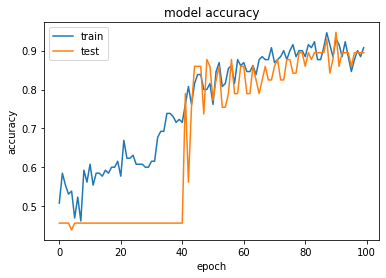
\includegraphics[height=0.35\textwidth]{images/chapter5/batch_256_100_epoch.png} &
        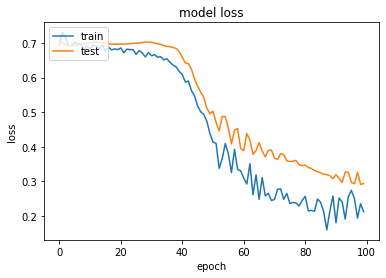
\includegraphics[height=0.35\textwidth]{images/chapter5/batch_256_100_epoch_loss.png}\\
        (a) & (b)\\
    \end{tabular}
    \label{fig:Resultados de entrenamiento con un batch-size de 256 y 100 epochs}
    \caption{Resultados de entrenamiento del modelo usando una GPU TeslaK80 con un batch-size de 256 y 100 epochs (a) Rendimiento del modelo en acierto. (b) Rendimiento del modelo en pérdida}
\end{figure}

\begin{figure}
    \centering
    \begin{tabular}{cc}
        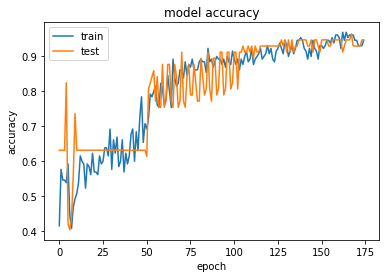
\includegraphics[height=0.35\textwidth]{images/chapter5/batch_256_175_epoch.png} &
        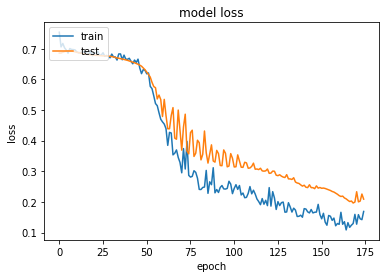
\includegraphics[height=0.35\textwidth]{images/chapter5/batch_256_175_epoch_loss.png}\\
        (a) & (b)\\
    \end{tabular}
    \label{fig:Resultados de entrenamiento con un batch-size de 256 y 175 epochs}
    \caption{Resultados de entrenamiento del modelo usando una GPU TeslaK80 con un batch-size de 256 y 175 epochs (a) Rendimiento del modelo en acierto. (b) Rendimiento del modelo en pérdida}
\end{figure}

\begin{figure}
    \centering
    \begin{tabular}{cc}
        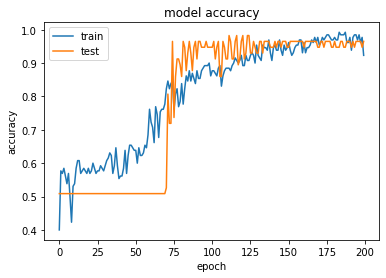
\includegraphics[height=0.35\textwidth]{images/chapter5/batch_256_200_epoch.png} &
        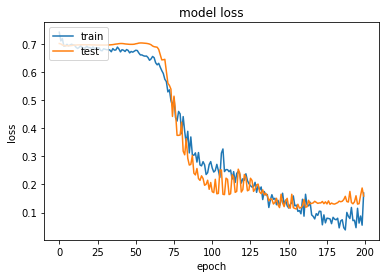
\includegraphics[height=0.35\textwidth]{images/chapter5/batch_256_200_epoch_loss.png}\\
        (a) & (b)\\
    \end{tabular}
    \label{fig:Resultados de entrenamiento con un batch-size de 256 y 200 epochs}
    \caption{Resultados de entrenamiento del modelo usando una GPU TeslaK80 con un batch-size de 256 y 100 epochs (a) Rendimiento del modelo en acierto. (b) Rendimiento del modelo en pérdida}
\end{figure}


\section{Rendimiento en fase de inferencias}\label{sec:ren-dimiento-en-fase-de-inferencias}
En cuanto a los tiempos de inferencia, la diferencia es notable entre OpenVINO y TensorFlow.
Los resultados se presentan haciendo uso de una muestra de 16.000 ejecuciones de inferencia en el entorno de producción de la aplicación, tanto para los entornos con OpenVINO, como para TensorFlow.
La unidad de cálculo principal es el procesador, siendo su modelo un Intel Xeon (Cascada Lake) con una frecuencia de 2.8 GHz de base y un turbo hasta 3.4 GHz.
Se han probado distintas configuraciones de este procesador, tanto en su versión de 2 núcleos físicos (4 virtuales), como en la de 4 núcleos físicos (8 virtuales).
La memoria RAM utilizada varía de 4 GB en su primera versión junto con el procesador de 2 núcleos físicos a 8 GB en la versión de 4 núcleos físicos.

En la Tabla\ref{tab:Comparativa de tiempo de inferencia con OpenVINO y TensorFlow} se puede observar como la media de inferencia a lo largo de las 16.000 muestras tomadas
es de 200 ms para TensorFlow y 4 ms para OpenVINO lo que supone una velocidad de inferencia 50 veces superior de OpenVINO frente a TensorFlow. También podemos visualizar en la Tabla~\ref{tab:Comparativa de tiempo de inferencia con OpenVINO y TensorFlow con distinto hardware} que el tiempo total de inferencia que incluye la latencia del servidor web, los pipelines de procesamiento del entorno y la propia inferencia, es inferior al segundo en ambos casos.
Y se reduce aún más en OpenVINO debido a la rapidez de su red de inferencia y la simplicidad con la que se implementa.
Al contrario que TensorFlow, no necesita ningún otro tipo de servicio adicional más que la API de alto rendimiento, que funciona como una librería almacenada de manera local en el sistema operativo.

\begin{table}[ht]
    \begin{center}
        \begin{tabular}{| c | c | c |}
            \hline
            inference\_engine & avg\_inference\_seconds & avg\_seconds\_total \\ \hline
            TensorFlow & 0.215 & 0.502 \\
            OpenVINO & 0.004 & 0.098 \\ \hline
        \end{tabular}
        \caption{Comparativa de tiempo de inferencia con OpenVINO y TensorFlow.}
        \label{tab:Comparativa de tiempo de inferencia con OpenVINO y TensorFlow}
    \end{center}
\end{table}

\begin{table}[ht]
    \begin{center}
        \begin{tabular}{| c | c | c | c | c | c |}
            \hline
            inference\_engine & physical\_core & system\_memory & avg\_inference\_seconds & avg\_seconds\_total \\ \hline
            TensorFlow & 4 & 7.00GB & 0.066 & 0.188 \\
            OpenVINO & 4 & 7.00GB & 0.003 & 0.1 \\
            OpenVINO & 2 & 3.46GB & 0.005 & 0.097 \\
            TensorFlow & 2 & 3.46GB & 0.364 & 0.816 \\ \hline
        \end{tabular}
        \caption{Comparativa de tiempo de inferencia con OpenVINO y TensorFlow con distinto hardware.}
        \label{tab:Comparativa de tiempo de inferencia con OpenVINO y TensorFlow con distinto hardware}
    \end{center}
\end{table}

Las distintas configuraciones hardware también revelan que el consumo de memoria del sistema de inferencia de TensorFlow afecta al rendimiento de la aplicación, mejorando mucho su rendimiento con un hardware más potente.
OpenVINO, por el contrario, mantiene resultados similares con un hardware de bajo coste.
TensorFlow mejora en 5 veces la velocidad de inferencia pasando de un procesador de 2 núcleos y 4 GB de RAM a uno de 4 núcleos y 8 GB de RAM teniendo un tiempo de 360 ms con el primero y 66 ms con el segundo, lo que denota que el consumo de su servicio de inferencia requiere de un hardware más caro. Del mismo modo mejora 8 veces su tiempo de inferencia total con la mejora del hardware pasando de 800 ms a 97 ms.


Se han configurado los distintos servidores web para que empleen todos los núcleos del procesador de manera concurrente, de modo que la capacidad de procesamiento de peticiones sea la máxima posible.
En la Tabla~\ref{tab:Comparativa de tiempo de inferencia con OpenVINO y TensorFlow con distinto framework web} podemos contemplar que OpenVINO se mantiene estable con ambos framework, con un ligero aumento de la latencia haciendo uso de fastapi.
TensorFlow se comporta mucho mejor con flask, mejorando en 4 veces su tiempo de inferencia en la red, pasando de 348 ms con fastapi a 83 ms con flask y 3.7 veces en el tiempo total de ejecución teniendo un rendimiento de 700 ms con fastapi a 200 ms con flask. Flask es un servidor web con los mínimos componentes para funcionar, pero configurado de la manera correcta puede ser el framework idóneo para realizar una tarea específica.
En este caso, la complejidad del servicio de TensorFlow convive mejor con un framework web sin demasiados componentes adicionales.
Los componentes que proporciona fastapi como un sistema de logging detallado de las ejecuciones y algunas características adicionales para el desarrollador, pueden ocasionar cierto aumento de la latencia en los tiempos.
Aun así, cuando la fiabilidad es uno de los requisitos y objetivos principales, estas mejoras pueden valer la pena a la hora de escalar nuestra aplicación.

\begin{table}[ht]
    \begin{center}
        \begin{tabular}{| c | c | c | c |}
            \hline
            inference\_engine & web\_engine & avg\_inference\_seconds & avg\_seconds\_total \\ \hline
            OpenVINO & Flask & 0.004 & 0.094 \\
            OpenVINO & FastApi & 0.005 & 0.103 \\
            TensorFlow & Flask & 0.083 & 0.212 \\
            TensorFlow & FastApi & 0.348 & 0.792 \\ \hline
        \end{tabular}
        \caption{Comparativa de tiempo de inferencia con OpenVINO y TensorFlow con distinto framework web.}
        \label{tab:Comparativa de tiempo de inferencia con OpenVINO y TensorFlow con distinto framework web}
    \end{center}
\end{table}

En general, fastapi requiere de un hardware más potente para sacar su máximo rendimiento, mientras que con una framework minimalista como flask podemos optar por reducir costes en hardware sin penalizar demasiado el rendimiento.
En la Tabla\ref{tab:Comparativa de tiempo de inferencia con OpenVINO y TensorFlow con distinto hardware y servidor web} podemos ver el rendimiento según hardware, servidor web y sistema de inferencia utilizado.

\begin{table}[ht]
    \begin{center}
        \small
        \begin{tabular}{ | c | c | c | c| c | c | c |}
            \hline
            engine & cores & framework & memory & avg\_inference\_seconds & avg\_seconds\_total \\ \hline
            OpenVINO & 2 & 3.46GB & FastApi & 0.006 & 0.104 \\
            OpenVINO & 4 & 7.00GB & FastApi & 0.004 & 0.102 \\
            TensorFlow & 2 & 3.46GB & FastApi & 0.608 & 1.349 \\
            TensorFlow & 4 & 7.00GB & FastApi & 0.087 & 0.235 \\
            OpenVINO & 2 & 3.46GB & Flask & 0.004 & 0.09 \\
            OpenVINO & 4 & 7.00GB & Flask & 0.003 & 0.098 \\
            TensorFlow & 2 & 3.46GB & Flask & 0.12 & 0.284 \\
            TensorFlow & 4 & 7.00GB & Flask & 0.045 & 0.141 \\ \hline
        \end{tabular}
    \end{center}
    \caption{Comparativa de tiempo de inferencia con OpenVINO y TensorFlow con distinto hardware y servidor web.}
    \label{tab:Comparativa de tiempo de inferencia con OpenVINO y TensorFlow con distinto hardware y servidor web}
\end{table}


El número total de aciertos de clasificación asciende a 1566 registros de un total de 16000, teniendo así un porcentaje de acierto general
del 97\%. Con un recuento de 108 fallos en la red TensorFlow y 226 en OpenVINO.
Todos los resultados y registros se encuentran en el repositorio oficial del trabajo en GitHub\footnote{\url{https://github.com/A-Ortiz-L/multispectral-imaging-cnn-final-degree-work/tree/master/result/snapshot}}.


\section{Costes del proyecto}\label{sec:costes-del-proyecto}
A continuación se presentan los costes del proyecto de toda la plataforma de producción.
Estos costes han sido recogidos haciendo uso de la calculadora de precios de Google\footnote{\url{https://cloud.Google.com/products/calculator?hl=es}}.

\begin{itemize}
    \item Máquina virtual 4 vCPUs, 3,6 GB 6.80 dólares por un uso de 24 horas, que fue el tiempo utilizado para realizar pruebas de concepto y cargas en este trabajo.
    \item Máquina virtual 4 vCPUs, 3,6 GB 3.40 dólares por un uso de 24 horas, que fue el tiempo real consumido para este servicio.
    \item BigQuery, con un coste de 0 dólares para un almacenamiento de 1 GB de tablas en la base de datos, 1GB de procesamiento en tiempo real y 1GB de trabajos SQL al realizar los análisis de resultados.
    \item Pub/Sub con un coste total de 0 dólares, ya que su uso entraba dentro del rango gratuito del servicio.
    \item Cloud Functions, con un coste total de 0 dólares, haciendo uso de la modalidad gratuita, que permite hasta 2 millones de llamadas al mes.
\end{itemize}